%%%%%%%%%%%%%%%%%%%%%%%%%%%%%%%%%%%%%%%%%%%%%%%%%%%%%%%%%%%%%%%%%%%%%%%%%%%%%%%%


%\documentclass[letterpaper, 10pt, conference]{IEEEtran}
\documentclass[letterpaper, 10pt, conference]{ieeeconf}
\IEEEoverridecommandlockouts
\overrideIEEEmargins 
\usepackage{tikz}
\usetikzlibrary{calc,decorations.markings,arrows}
\usepackage{tikz-timing}
\usepackage[top=1in,bottom=1in,right=1in,left=1in]{geometry}
\usepackage{amsmath}
\usepackage{xifthen}
\usepackage{amsfonts}
\usepackage{tabu}
\usepackage{graphicx}
\usepackage[font=small]{caption}
\usepackage{subcaption}
\usepackage{cite}
\usepackage{xspace}
\usepackage{subfiles}
\usepackage{url}

% Packages for including pseudo-code
\usepackage{algorithmicx}
\usepackage{algorithm}
\usepackage{algpseudocode}

% Nice Little macro for adding a comment box. Include incrementing comment numbers.
\newcounter{comcount}
\setcounter{comcount}{0}
\newcommand{\mycomment}[1]
{
\refstepcounter{comcount}
\smallskip\noindent\fbox{\parbox{\linewidth}{\emph{Comment \arabic{comcount}} : \small{#1}}} 
}

\newcommand{\spx}{\mathcal{S}}

%
%Once I break this in to multiple sections, each section will be added with:
%	\subfile{filename}
%In those other files, I have as preamble:
%	\documentclass[main.tex]{subfiles}
%

\title{\LARGE \bf
A Stick-Slip Omnidirectional Drive-Train for Low-Cost Swarm Robotics: Mechanism, Calibration, and Control
}

\author{John Klingner, Anshul Kanakia, Nicholas Farrow, Dustin Reishus and Nikolaus Correll%
\thanks{Department of Computer Science,
University of Colorado at Boulder,
 Boulder, CO 80309,
{\tt\small firstname.lastname{@}colorado.edu}}%
}

\begin{document}
\maketitle


%%%%%%%%%%%%%%%%%%%%%%%%%%%%%%%%%%%%%%%%%%%%%%%%%%%%%%%%%%%%%%%%%%%%%%%%%%%%%%%%
\begin{abstract}
We present an omni-directional drive train for swarm robotic platforms that relies on low-cost vibration motors. We describe a mechanism and controller to achieve full 3-DoF motion on the plane. The proposed approach does not require the motors to be in phase, and overcomes differences in manufacturing by a hardware-in-the-loop auto-calibration routine based on the Nelder-Mead algorithm, which issues motion commands via infrared and records the resulting trajectories using an off-the-shelf webcam. We show convergence results of the calibration routine and sample trajectories of the swarm robotic platform ``Droplet'' demonstrating turning and omni-directional drive.   
\end{abstract}

%\keywords{Swarm robotics, low-cost, hopping robot, bristle-bot principle}


%%%%%%%%%%%%%%%%%%%%%%%%%%%%%%%%%%%%%%%%%%%%%%%%%%%%%%%%%%%%%%%%%%%%%%%%%%%%%%%%
\section{Introduction}
We present a low-cost miniature robot drive-train that approximates omni-directional motion using three vibration motors. Classically, miniature robotic platforms such as r-one \cite{mclurkin2013low}, Jasmine \cite{jasmine} and Alice \cite{alice} require geared motors, which are expensive and difficult to miniaturize. The proposed drive-train is a variant of the ``stick-slip'' actuator that has been introduced in \cite{breguet1998stick}, and has been shown to be particularly attractive for high precision movements \cite{brufau2005micron,chu2006novel,martel2001three,martel2005fundamental,eigoli2012locomotion} and force control \cite{vartholomeos2008analysis}.   

Whereas stick-slip actuators traditionally require changing their length, e.g., using piezo ceramics,  \cite{breguet1998stick, martel2005fundamental}, a similar effect can be achieved using a vibration motor, an effect well- known from the ``Bristle-bot'' series of toys. The simplicity and availability of this actuator  has led to its use on low-cost miniature robot platforms such as the Kilobots \cite{rubenstein2012kilobot} based on the design presented in \cite{Vartholomeos2006}, which approximates the dynamics of a differential wheel platform (see also \cite{spartali2013speed} for additional analysis). Achieving fully holonomic motion on the plane requires at least three vibration motors, however. Whereas \cite{Vartholomeos2005} proposes a symmetric three motor design and its analysis, their approach requires all motors to be in phase, which is not feasible on a low-cost platform. This paper addresses these problems by presenting a design, controller and calibration routine that allows omnidirectional motion on a ping-pong ball sized robot ``Droplet'' (Figure \ref{Droplets}).

\begin{figure}[!htb]
	\centering
		\includegraphics[width=0.8\columnwidth]{./Images/Droplets.png}
	\caption{The Droplet swarm robotics platform. Two Droplets are shown, one with the cover removed. A penny is included for scale. The background is the floor of alternating power and ground strips from which the Droplets draw power.}
	\label{Droplets}
\end{figure}


%%%%%%%%%%%%%%%%%%%%%%%%%%%%%%%%%%%%%%%%%%%%%%%%%%%%%%%%%%%%%%%%%%%%%%%%%%%%%%%%
\section{The Droplet Swarm Robotic Platform}
The Droplets are an open-source swarm robotic platform, with source code and manufacturing information available online\footnote{\url{https://github.com/correlllab/cu-Droplet}}. 

Each Droplet is a spherical, roughly ping-pong ball sized robot with a radius of $2.2$cm and a flat bottom. They have three extended headers for legs located symmetrically around the robot. The legs are spaced 120 degrees apart, 15.1mm (0.595in) from the center. Mounted symmetrically opposite the legs are coin-type vibration motors (\emph{Hochar}) arranged as shown in Figure (\ref{fig:PWMs}). The  motors  are circular shaped, 10mm in diameter and 2.7mm thick, weigh 1.1g, rated at 3V DC, vibrate at 200$\pm$42 Hz, and of the type commonly used in cell phones and pagers. As locomotion is not their primary intent, the vibration motors used here have low manufacturing consistency and are inconsistent about both the direction in and frequency with which they spin.

\begin{figure}[!htb]
	\centering
	\subfile{motorLocations}
	\caption{An image of the Droplet's shell and vibration motors in place. The locations where the legs are mounted are labeled.}
	\label{fig:PWMs}
\end{figure}

The Droplets receive power from these legs through a floor with alternating strips of $+5V$ and $GND$. The Droplets use an Atmel Xmega128A3U microcontroller, along with H-bridge Allegro A3901 Dual Motor Drivers. Motors are controlled via this H-Bridge that is driven by a pulse-width modulated (PWM) signal generated by the microcontroller. This setup allows us to provide a series of precise pulses as well as changing the direction of rotation. A 6-directional infrared communication and range and bearing system \cite{farrow14} is also present on the Droplets.


%%%%%%%%%%%%%%%%%%%%%%%%%%%%%%%%%%%%%%%%%%%%%%%%%%%%%%%%%%%%%%%%%%%%%%%%%%%%%%%%
\section{Principle of Operation}

\subsection{Base Motion Principle}
A vibration motor is a DC motor with a mass on the shaft, such that the center of mass is not on the axis of rotation. Spinning the motor throws the mass around, causing motion of the entire motor body due to inertia. As the mass swings through its circular path, the motor experiences a force towards that mass. Over the course of a full rotation, the net force experienced by the motor is 0. This is illustrated in Figure \ref{motorDiagram}.

\begin{figure*}[!htb]
\centering
\subfile{singleDoFModel}
\caption{Simple 1DoF model of motion principle, from the side. Upwards motion of the motor creates upwards force, significantly reducing the friction between the two legs and the ground. Spinning the motor also results in a forward force, moving the platform forwards. Albeit completing the revolution creates a backwards force, friction also begins to inrease, resulting in an overall forward motion \cite{Vartholomeos2005}.}
\label{motorDiagram}
\end{figure*}

If we neglect friction, the platform will slide backwards and forwards due to the backwards and forwards forces from the mass, but experiences no net translation. With friction, the vertical forces of the mass become relevant. The downward force of gravity is mitigated by the upward force from the swinging mass. Crucially, this means that the total downward force experienced by the platform is lower while the mass is swinging upwards. Thus, the platform experiences reduced friction while the mass is swinging upwards. The direction of lateral magnitude during this period of reduced friction (or, the direction the motor is spinning) determines the direction of travel, see also \cite{Vartholomeos2005,Vartholomeos2006} for a mathematical treatment of this model. Figure~\ref{motorDiagram} illustrates this process. Note that the robot does not actually need to jump up, as long as the upward force sufficiently reduces static friction. 


\subsection{Motion Principle Applied to Droplets}
Combining the 1-DoF actuator described above with others to obtain a 3-DoF robotic platform is not trivial as it requires all motors to be in phase \cite{Vartholomeos2005}, and infeasible with low-cost hardware. Our proposed design deviates from \cite{Vartholomeos2005} by positioning our motors opposite, instead of above, the platform's legs as shown in Figure~\ref{DropletMotorDiagram}. With this configuration, the motor forces cause the platform to pivot about the opposite leg.

%With the simplifying assumption that the platform is a uniform mass, lets consider the forces applied to the platform as a single motor $m_i$ rotates. Since the platform touches the floor only with its three legs, it will be relevant to consider the downward force $f_i$ on each leg separately.

\begin{figure}[!htb]
\centering
\subfile{DropletDiagram}
\caption{Arrangement of vibration motors $m_0, m_1$ and $m_2$ and legs $l_0, l_1$ and $l_2$.}
\label{DropletMotorDiagram}
\end{figure}

%\subsubsection{Straight motion}
%\mycomment{Remove most of this subsection. Keep the last paragraph and justify it with ``words'' here.}
%Let us consider a single pivot caused by motor $i$ ($m_i$), about leg $i$ ($l_i$), of some small, positive radial distance $\theta_i$. This motion causes the center of the Droplet to trace $\theta_i$ of an arc about $l_i$. The length of the chord with the same endpoints as the arc, $C$, i.e. the distance traveled by the center of the Droplet, is given by:
%\begin{equation}\label{eq:arclength}
%C=2 L \sin\left(\frac{\theta_i}{2}\right)
%\end{equation}
%Where $L$ is the distance between the robot's center and leg; the radius of the arc. To break this displacement in to its $x$ and $y$ components, we first need to know the angles of the triangle made by the chord and the leg. We can get this using the law of sines:
%\begin{equation}
%x = \arcsin\left(\frac{L}{C}\sin(\theta)\right) 
%\end{equation}
%Inserting the arc length $C$ from \ref{eq:arclength} gives:
%\begin{align}
%x &=\arcsin\left(\frac{L\sin(\theta)}{2 L \sin(\frac{\theta}{2})}\right) \\
%\nonumber
%   &=\arcsin\left(\cos\left(\frac{\theta}{2}\right)\right)
%\end{align}
%
%Given this angle $x$, and the known angle between the Droplet's $x$\~axis and the leg ($\phi_1$), we can calculate the direction of the platform's displacement:
%%
%\begin{align}
%\delta x_a &= C \cos(\pi - x - \phi)\\
%\nonumber
%\delta y_a &= C \sin(\pi - x - \phi)
%\end{align}
%
%Note also that the orientation of the Droplet has changed by $\theta$. Next, consider a second pivot by $m_2$ of $-\theta$. By symmetry, we now have:
%%
%\begin{align}
%\delta x_b &= -C\cos(\pi -x -\phi)\\
%\nonumber
%\delta y_b &= C \sin(\pi - x - \phi)
%\end{align}
%%
%and the orientation has now changed by $-\theta$, putting the Droplet back in its original orientation. 

In practice, the proposed locomotion scheme only works with one motor being active at a time. In addition to the motor placement that allows pivoting, this assumption allows us to overcome the limitations of the motors being in phase as described in \cite{Vartholomeos2005}. Therefore, the robots are not moving straight, but crawl forward in a S-shape. In order to move straight, this requires an initial turn to counter the offset introduced by the S-shape. 

%The size of this error is a function of the arc of the step. As $\theta$ approaches $0$, so does the error. Similarly, when spinning each cycle of three motors doesn't leave us back at our exact original position, but it does bring us pretty close.

%By restricting ourselves to these small-pivot ``steps'', we avoid the requirements of precise balance and motor-phase synchronization that causes trouble with more direct implementations \cite{Vartholomeos2006}.

%To simplify, we focus on the platform moving in one of six directions: (0,180, $+/-$60, $+/-$120) degrees, as well as clockwise and counterclockwise rotation. It should be a straightforward extension to get arbitrary 3DoF motion by combining these directions.

\subsection{Forward and inverse kinematics}
We now attempt to map these stick-slip drivetrain kinematics to the more traditional kinematics of wheeled robots.

Whereas each pivot motion happens at the maximal speed of the platform, we can approximate the effective speeds $\theta_i$ by introducing delays of varying length after each microscopic pivot. Assuming that low-level control of $\theta_i$ and switching between pivot motions happens much faster than actual motion, we can reduce the proposed mechanism to a circular robot with three standard wheels, albeit without kinematic constraints, at the same location and orientation as the motors shown in Figure~\ref{DropletMotorDiagram} and retractable legs. Here, the absence of kinematic constraints lets the standard wheels skid frictionlessly in any direction, whereas the retractable legs allow to enable and disable pivot points, modeling the up and down movements of the platform. 

In this reduced model, each motor $m_0$, $m_1$, and $m_2$ controls the angular velocity $\dot{\theta}_0$, $\dot{\theta}_1$ and $\dot{\theta}_2$ around its associated pivot point opposite of the motor. This lets us derive the following forward kinematic equations in the robot coordinate frame $\dot{x}_r$, $\dot{y}_r$ and $\dot{\theta}_r$.
Here we assume the $y$-axis to be orthogonal to the spinning direction of motor 2, and the $x$-axis orthogonal to the $y$-axis, as seen in Figure~\ref{DropletMotorDiagram}
\begin{align}\label{eq:fwd}
\dot{x}_r & = -L \dot{\theta}_0 \cos(2 \pi / 3) + L \dot{\theta}_1 \sin(\pi / 6) + L \dot{\theta}_2\notag\\
\dot{y}_r & =  L \dot{\theta}_0 \sin(2 \pi / 3) - L \dot{\theta}_1 \cos(\pi / 6)\notag\\
\dot{\theta}_r & = \dot{\theta}_0 + \dot{\theta}_1 + \dot{\theta}_2
\end{align}
Here, we assume positive $\theta_i$ to be aligned with the direction of thrust of motor $m_i$ and each leg having distance $l$ from the motors. That is, if all motors spin in the same direction, they all contribute to $\dot{\theta}_r$ in the same way. Notice that motor 2 does not contribute to $\dot{y}_r$ as it spins orthogonally to the y-axis.

Equation \ref{eq:fwd} is a linear system with three unknowns, and we can solve for $\dot{\theta}_0$, $\dot{\theta}_1$ and $\dot{\theta}_2$:
\begin{align}\label{eq:ik}
\dot{\theta}_0 & = -\frac{\dot{x}_r}{L} + \frac{\dot{y}_r}{\sqrt{3}L} + \dot{\theta}_r\notag\\
\dot{\theta}_1 & = -\frac{\dot{x}_r}{L} - \frac{\dot{y}_r}{\sqrt{3}L} + \dot{\theta}_r\notag\\
\dot{\theta}_2 & = \frac{2 \dot{x}_r}{L} - \dot{\theta}_r
\end{align}

The rotational velocity values from \eqref{eq:ik} can now be transformed to motor values supplied to the Droplet to achieve desired motion in the $\{\dot{x}_r, \dot{y}_r, \dot{\theta}_r\}$ coordinate frame using auto-calibration techniques discussed in the following section.




%%%%%%%%%%%%%%%%%%%%%%%%%%%%%%%%%%%%%%%%%%%%%%%%%%%%%%%%%%%%%%%%%%%%%%%%%%%%%%%%
\section{Auto-Calibration}
Additional challenges arising from low-cost hardware is that achieving equal step sizes requires tedious calibration.
It is possible to calibrate each platform manually, by setting values and eyeballing how well they work. As stated earlier, however, this platform is motivated by a desire for low-cost, large scale robot swarms.  Manual calibration of a swarm of thousands of robots would be completely impractical, and so we automate the process.

\subsection{Experimental Setup}
The motors are kept at a fixed $100\%$ duty cycle. Each step, we turn a motor on for a fixed amount of time, $t_{\text{on}}$, plus some offset, $\tau$,  which varies for each motor direction. Next, all motors are off for a fixed amount of time, $t_{\text{off}}$. Figure~\ref{fig:pwmSignals} shows this in more detail. We denote the vector of calibration values for each motor direction $\vec{\tau}$. Calibration is done by changing the $\vec{\tau}$ values such that the pivot induced by the motors is the same. These values are integers of magnitude $^1/_{32}$$ms$. For our platform, $t_{\text{on}}$ is $30ms$, which was determined to be the minimum amount of time required to induce pivoting for a typical motor. Similarly, $t_{\text{off}}$ is the time required for vibrations of the system to settle---a shorter off time causes platform instability.

\begin{figure}[!htb]
\centering
\subfile{PWMfigure}
\caption{The PWM signals for motion in the 0 direction. If both forward (FW) and reverse (RV) are high, the motor is braking. If only one signal is high, the motor rotates in that direction. Thus, to spin forward we keep FW high and drop RV low when we want the motor to actually spin.}
\label{fig:pwmSignals}
\end{figure}

Data is collected using a high resolution USB camera\footnote{Microsoft LifeCam Cinema}, and motion-tracking software RoboRealm~\cite{RoboRealm}. A fiducial marking is secured to the top of the platform to aid in tracking and orientation calculations (Figure~\ref{fig:expsetup}). Specifically, we collect the global position and orientation of the Droplet in each frame.

To update the Droplet's calibration settings, we find the least-squares best-fit circle of the collected coordinates. Specifically, the circle's radius and whether that circle's center is to the Droplet's left or right. While calibrating for walking straight, we optimize for maximizing the radius of the fitted circle (if the Droplet traveled perfectly straight, the radius would by infinite). While calibrating for spinning, we optimize for minimizing the radius of the fitted circle (a perfect spin would have radius 0).

We communicate with and control the platform through a serial to IR transmitter. 

\begin{figure}[!htb]
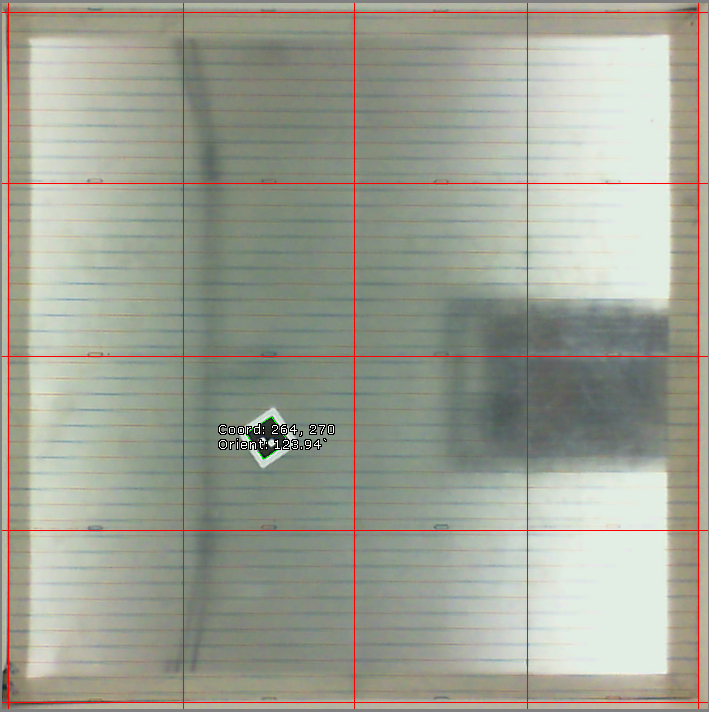
\includegraphics[width=\linewidth]{images/cameraView}
\caption{View from the overhead camera onto the Droplet equipped with a fiducial marker that can be recognized by RoboRealm.\label{fig:expsetup}} 
\end{figure}

\subsection{Calibration Method}
\begin{algorithm}
\caption{Automated method for calibrating an individual Droplet's rotational motion}
\begin{algorithmic}
	\Function{Auto\_Calibrate}{$dir, \alpha, \beta$}		
		\State $\spx \gets$ init\_simplex\_guess()
		\State $[\tau^*_1,\tau^*_2, \tau^*_3] \gets$ Nelder\_Mead($\spx, dir, \alpha, \beta$) 
		\State write\_to\_memory($id_{robot}, dir, \tau^*_1,\tau^*_2, \tau^*_3$)
	\EndFunction
	\Function{Nelder\_Mead}{$\spx, dir, \alpha, \beta$}
		\State $radii \gets$ new list()
		\State $v \gets$ new list()
		\For{$\vec{\tau}$ in $\spx$}
			\State $radii$.push(get\_robot\_spin\_circle\_est($\vec{\tau}, dir$))
			\State $v$.push(get\_robot\_spin\_vel\_est($\vec{\tau}$))
		\EndFor
		\State $\spx' \gets$ new\_simplex\_est($\spx, radii, v, dir, \alpha, \beta$)
		\If{within\_tolerence($\spx', radii, v$)}
			\State \Return best\_values($\spx'$)
		\Else
			\State Nelder\_Mead($\spx', \alpha, \beta$)
		\EndIf
	\EndFunction
\end{algorithmic}\label{alg:spx}
\end{algorithm}

We use the popular Nelder-Mead Simplex algorithm \cite{NelderMead} to calibrate motor parameters for spinning in a given direction (clockwise or anti-clockwise), as seen in Alg.(\ref{alg:spx}). 

The simplex algorithm attempts to minimize the radius of the circle that the Droplet makes while rotating while, at the same time, maximize the speed of rotation. The objective function used by the algorithm is,
\begin{equation}
\text{(max.)} \quad -\alpha.r_{circ}(\tau_1, \tau_2, \tau_3) + \beta.v_{rot}(\tau_1, \tau_2, \tau_3)\label{eq:maxcal}
\end{equation}
where $\alpha$ and $\beta$ are weighting constants such that $\alpha > \beta$, as we prefer motor values that minimize circle radius over rotational speed.

Each of the four vertices in the simplex is a set of three motor calibration parameters, i.e., $\spx = \{\vec{\tau}^1, \vec{\tau}^2, \vec{\tau}^3, \vec{\tau}^4\}$, where $\vec{\tau}^i = \{\tau^i_1, \tau^i_2, \tau^i_3\}$. The algorithm attempts to provide iteratively better motor control parameters by solving the optimization problem \eqref{eq:maxcal} until a sufficiently accurate set of parameters is provided that falls within the desired tolerances of rotational circle radius and velocity.

Additionally, this method identifies which motors are `flipped'---i.e., which motors spin opposite from what's expected. This is because having the motor directions wrong results in a large radius. Once we have clockwise spin calibrated, this is equivalent to having three matched pivot sizes for the motors' clockwise spins. To finish calibrating, we just need to find counterclockwise values that match the clockwise ones. This is done for each motor independently by having the Droplet walk straight in a direction. Now, we want to maximize the radius of the the circle traced by the Droplet. As the Droplet improves straight-line motion accuracy, the radius of the circle transcribed by its motion approaches $\infty$. A binary search is performed over the space of possible clockwise values for each motor.

Note that since the Nelder-Mead algorithm also treats flipped motors, it's possible for it to find a minima with all motors flipped, spinning in the counterclockwise direction. The rest of the algorithm is performed symmetrically in this case.

%%%%%%%%%%%%%%%%%%%%%%%%%%%%%%%%%%%%%%%%%%%%%%%%%%%%%%%%%%%%%%%%%%%%%%%%%%%%%%%%
\section{Results}

\subsection{Calibration}
We performed calibration for four different Droplets. Figure \ref{fig:radiiConverging} shows convergence of the optimization routine, and Table~\ref{DropletValueTable} shows a sample of calibrated values. This demonstrates the variability of the individual robots.

\begin{figure}[!htb]
\centering
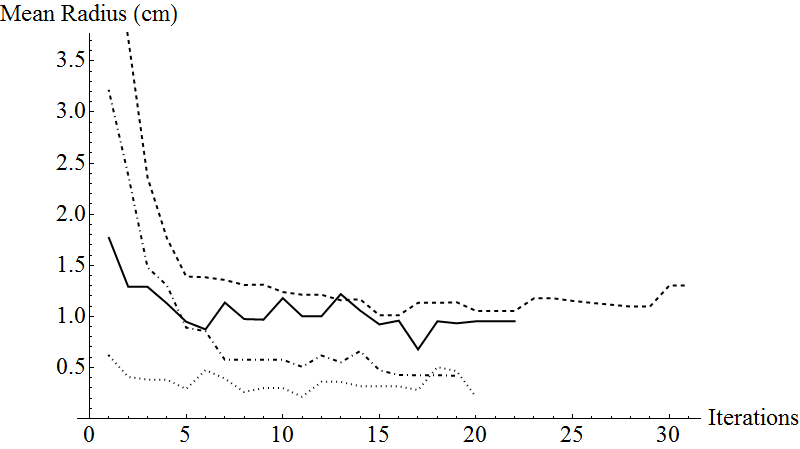
\includegraphics[width=\linewidth]{Images/radiiConverging.png}
\caption{The mean of the best three points of the simplex after each pass through the Nelder-Mead optimization loop, shown for four different Droplets. After the optimization converges or a particularly good value is found, the motors are set to the best of all settings tested.}
\label{fig:radiiConverging}
\end{figure}

\begin{table}[!htb]
\centering
\begin{tabular}{r|c|c|c|c|c|c}
 ID & $m_0$ & $-m_0$ & $m_1$ & $-m_1$ & $m_2$ & $-m_2$ \\
\hline
15 & 68 & -1 & 56 & -5 & \emph{40} & \emph{0}\\ 
18 & 84 & -89 & 84 & 202 & \emph{128}  & \emph{290}\\
11 & -96 & 83 & 64 & 62 & -289 & 55 \\
\end{tabular}
\caption{Sample of calibrated values for specific Droplets. \emph{Italicized} values indicate that that particular motor was flipped. $-m$ is used to indicate the reverse value for that motor.}
\label{DropletValueTable}
\end{table}

\subsection{Motion}
%In order to verify that the Droplets indeed walk in a S-shape wiggling motion, we recorded the path of an individual Droplet with a high-speed camera (Casio Exilim ZR200). A snapshot of the resulting trajectory is shown in Figure XXXX.
For a more robust demonstration of the calibrated Droplet's performance, we performed two additional experiments. Figure~\ref{fig:squareWalk} shows two attempts of a Droplet walking in a square pattern, produced by walking forward and turning 90 degrees to the right repeatedly. For the solid trial, with nominal square size of $8cm$, this resulted in a final position error of $2.75cm$ and a final orientation error of $27$ degrees. For the dashed trial, with nominal size $6.5cm$, this resulted in a final position error of $1.4cm$ and final orientation error of $39$ degrees.

\begin{figure}[!htb]
\centering
\includegraphics[width=0.9\linewidth]{Images/DropletWalksSquare}
\caption{Two attempts (solid, dashed) of a calibrated Droplet walking in a square, combing straight motion with a rotation.}
\label{fig:squareWalk}
\end{figure}

Figure~\ref{fig:triangleWalk} shows two attempts of a Droplet walking a triangle pattern. This is done without rotations, using the two degrees of translational freedom. Both trials have a nominal side length of $6cm$. The final position errors were $3.28cm$ and $2.77cm$ for the solid and dashed paths respectively.

\begin{figure}[!htb]
\centering
\includegraphics[width=0.9\linewidth]{Images/DropletWalksTriangle}
\caption{Two attempts (solid, dashed) of a calibrated Droplet walking in a triangle without rotation. The two attempts are aligned so that the Droplet}
\label{fig:triangleWalk}
\end{figure}

%%%%%%%%%%%%%%%%%%%%%%%%%%%%%%%%%%%%%%%%%%%%%%%%%%%%%%%%%%%%%%%%%%%%%%%%%%%%%%%%
\section{Discussion}
The proposed control scheme relies on running the vibration motors at full speed for a brief moment of time. What this timing should be is an outcome of the optimization routine. While this approach leads to acceptable results and a wide range of possible motions, it is not necessarily optimal with respect to speed and power consumption. For example, we could also vary the voltage provided to the motors using a high-frequency PWM signal, which might lead to even better speed/power performance. We wish to explore this and other control schemes in future work, though increasing the search space is generally undesirable in a hardware-in-the-loop optimization scheme.  

Calibrating the Droplets via an overhead camera and off-the-shelf computer vision software allows to obtain results quickly and potentially scales to calibration of multiple robots at the same time. An alternative approach would be to rely on the Droplets' range-and-bearing system \cite{farrow14} which would potentially allow a large number of Droplet to calibrate in parallel without additional hardware.

The proposed forward and inverse kinematics are an approximation as the robots do not move in straight lines, but using a sequence of pivoting steps. While this effect is negligible over distances in the order of the robot's diameter, it is prohibitive to reach the accuracies that the stick-slip drive is capable off. For example, when ``spinning in place'', the robots' coordinate system moves in a radius in the order of millimeters. In the future, we wish to explore motion planning techniques to achieve sub-millimeter accuracy by combining a sequence of motion, much like a knight on a chess board needs to do to reach a neighboring cell. 

Similarly, the inverse kinematics solutions in Equation \ref{eq:ik} provide correct, but possibly sub-optimal solutions. For example, solving for $\dot{x_r}=0$, $\dot{y}=0$ and $\dot{\theta}_r$ arbitrary, results in $\dot{\theta}_0=\dot{\theta}_r$, $\dot{\theta}_1=\dot{\theta}_r$ and $\dot{\theta}_2=-\dot{\theta}_r$. Albeit these values will let the robot spin in place with speed $\dot{\theta}_r$, these results are far from the optimal values $\dot{\theta}_0=\dot{\theta}_1=\dot{\theta}_2=\frac{\dot{\theta}_r}{3}$. 

\section{Conclusion}
We presented an omni-directional drive train and miniature robotic platform that relies on low-cost vibration motors. We have shown how we can overcome challenges with synchronization and manufacturing variability, which have thus far prevented this approach from practical viability. 

Whereas the proposed auto-calibration allows us to make up for manufacturing variability, it still requires significant manual labor to calibrate individual platforms, which is tedious for swarms with thousands of robots that we envision. In the future, we will therefore investigate methods to calibrate robots collaboratively and online.  

\section*{Acknowledgments} We thank Dr.\ Timothy Caldwell for helpful discussion on suitable optimization methods. 
This work has been supported by NSF award \#1150223 and a CI fellowship to D. Reishus.


\bibliographystyle{ieeetr}
\bibliography{mybibfile}

\end{document}

